\section{REST Interface}
This REST APIs were generated using \textit{Swagger Editor} and the functionalities implemented are:

\begin{itemize}
	\item \textbf{GET}:
		\subitem \textit{containers/} : Retrieve the list of all containers with their informations \footnote{The Swagger\_server computes the total number of actives hosts, but if some of them go down the GET operation retrieves only the ones that respond within a lap of time equal to 4 seconds. If all of the hosts answer to the request in a shorter time, the REST interface stops wait for answers and send the list of all containers back to the user}. The \textit{response} is a list of containers containing for each one its hostname, its name, its status and if it is monitored or not. The number of container in the cluster is computed at runtime in order to wait all their responses, if some of them doesn't replay within four seconds the operation concludes sending the information received up to that time.
	\item \textbf{POST}:
		\subitem \textit{containers/\{hostname\}/\{containerName\}} : Monitor the container specified in the path
	\item \textbf{DELETE}:
		\subitem \textit{containers/\{hostname\}/\{containerName\}} : Unmonitor the container specified in the path
	\item \textbf{PUT}:
		\subitem \textit{/threshold} : Update the packet loss threshold used in the Agent. The value is specified in the body of the request and its type is \textit{double}.
\end{itemize}

\noindent The REST Interface makes use also of a model for specifying the structure of a Container, which is the following\footnote{the asterisk indicates that the attribute must be set}:

\begin{figure}[H]
	\begin{subfigure}{\textwidth}
	\centering
		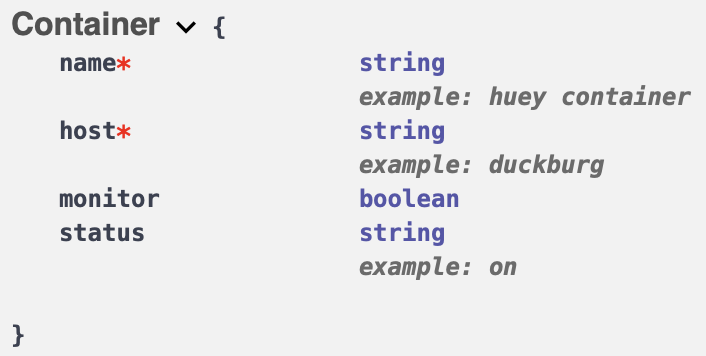
\includegraphics[width=0.9\linewidth]{img/container.png} 
	\end{subfigure}
\end{figure}